%%%%%%%%%%%%%%%%%%%%%%%%%%%%%%%%%%%%%%%%%
% Beamer Presentation
% LaTeX Template
% Version 1.0 (10/11/12)
%
% This template has been downloaded from:
% http://www.LaTeXTemplates.com
%
% License:
% CC BY-NC-SA 3.0 (http://creativecommons.org/licenses/by-nc-sa/3.0/)
%
%%%%%%%%%%%%%%%%%%%%%%%%%%%%%%%%%%%%%%%%%

%----------------------------------------------------------------------------------------
%	PACKAGES AND THEMES
%----------------------------------------------------------------------------------------

\documentclass{beamer}

\mode<presentation> {

% The Beamer class comes with a number of default slide themes
% which change the colors and layouts of slides. Below this is a list
% of all the themes, uncomment each in turn to see what they look like.

%\usetheme{default}
%\usetheme{AnnArbor}
%\usetheme{Antibes}
%\usetheme{Bergen}
%\usetheme{Berkeley}
%\usetheme{Berlin}
%\usetheme{Boadilla}
%\usetheme{CambridgeUS}
%\usetheme{Copenhagen}
%\usetheme{Darmstadt}
%\usetheme{Dresden}
%\usetheme{Frankfurt}
%\usetheme{Goettingen}
%\usetheme{Hannover}
%\usetheme{Ilmenau}
%\usetheme{JuanLesPins}
%\usetheme{Luebeck}
\usetheme{Madrid}
%\usetheme{Malmoe}
%\usetheme{Marburg}
%\usetheme{Montpellier}
%\usetheme{PaloAlto}
%\usetheme{Pittsburgh}
%\usetheme{Rochester}
%\usetheme{Singapore}
%\usetheme{Szeged}
%\usetheme{Warsaw}

% As well as themes, the Beamer class has a number of color themes
% for any slide theme. Uncomment each of these in turn to see how it
% changes the colors of your current slide theme.

%\usecolortheme{albatross}
%\usecolortheme{beaver}
%\usecolortheme{beetle}
%\usecolortheme{crane}
%\usecolortheme{dolphin}
%\usecolortheme{dove}
%\usecolortheme{fly}
%\usecolortheme{lily}
%\usecolortheme{orchid}
%\usecolortheme{rose}
%\usecolortheme{seagull}
%\usecolortheme{seahorse}
%\usecolortheme{whale}
%\usecolortheme{wolverine}

%\setbeamertemplate{footline} % To remove the footer line in all slides uncomment this line
%\setbeamertemplate{footline}[page number] % To replace the footer line in all slides with a simple slide count uncomment this line

%\setbeamertemplate{navigation symbols}{} % To remove the navigation symbols from the bottom of all slides uncomment this line
}

\usepackage{graphicx} % Allows including images
\usepackage{booktabs} % Allows the use of \toprule, \midrule and \bottomrule in tables
\usepackage{mleftright}
\usepackage{algorithm}
\usepackage{algpseudocode}

%----------------------------------------------------------------------------------------
%	TITLE PAGE
%----------------------------------------------------------------------------------------

\title[t-SVD]{Tensor Singular Value Decomposition and Composition} % The short title appears at the bottom of every slide, the full title is only on the title page

\author{Miao Yin} % Your name
\institute[] % Your institution as it will appear on the bottom of every slide, may be shorthand to save space
{
Rutgers University \\ % Your institution for the title page
\medskip
\textit{miao.yin@rutgers.edu} % Your email address
}
\date{\today} % Date, can be changed to a custom date

\begin{document}

\begin{frame}
\titlepage % Print the title page as the first slide
\end{frame}

\begin{frame}
\frametitle{Overview} % Table of contents slide, comment this block out to remove it
\tableofcontents % Throughout your presentation, if you choose to use \section{} and \subsection{} commands, these will automatically be printed on this slide as an overview of your presentation
\end{frame}

%----------------------------------------------------------------------------------------
%	PRESENTATION SLIDES
%----------------------------------------------------------------------------------------

%------------------------------------------------
\section{Tensor Singular Value Decomposition (t-SVD)} % Sections can be created in order to organize your presentation into discrete blocks, all sections and subsections are automatically printed in the table of contents as an overview of the talk
%------------------------------------------------

\begin{frame}{Notation}
$$
\mathbf{A}^{(j)}\equiv\mathcal{A}(:,:,j),~~~~\hat{\mathcal{A}} = \texttt{fft}(\mathcal{A}, [], 3)
$$
$$
\texttt{bcirc}(\mathcal{A})=\left[
  \begin{matrix}
   \mathbf{A}^{(1)} & \mathbf{A}^{(n)} & \mathbf{A}^{(n-1)} & \cdots & \mathbf{A}^{(2)} \\
   \mathbf{A}^{(2)} & \mathbf{A}^{(1)} & \mathbf{A}^{(n)} & \cdots & \mathbf{A}^{(3)} \\
   \vdots & \vdots & \vdots & \ddots & \vdots \\
    \mathbf{A}^{(n)} & \mathbf{A}^{(n-1)} & \cdots & \mathbf{A}^{(2)} & \mathbf{A}^{(1)}
  \end{matrix}
  \right]
$$
$$
\texttt{unfold}(\mathcal{A})=\left[
  \begin{matrix}
    \mathbf{A}^{(1)} \\
    \mathbf{A}^{(2)} \\
    \vdots \\
    \mathbf{A}^{(n)}
  \end{matrix}
\right], ~~~~~~~~\texttt{fold}(\texttt{unfold}(\mathcal{A}))=\mathcal{A}
$$
\end{frame}

%------------------------------------------------

\begin{frame}{t-Product}
\begin{block}{Definition. t-product}
Let $\mathcal{A}$ be $n_1 \times n_2 \times n_3$ and $\mathcal{B}$ be $n_2 \times n_4 \times n_3$. Then the t-product $\mathcal{A} * \mathcal{B}$ is the $n_1 \times n_4 \times n_3$ tensor 
$$\mathcal{A}*\mathcal{B}=\texttt{fold}(\texttt{bcirc}(\mathcal{A})\cdot\texttt{unfold}(\mathcal{B})).$$
\end{block}
\textbf{Example 1}. Let $\mathcal{A}\in\mathbb{R}^{3\times 2 \times 2}$ with frontal faces
$$
%\renewcommand\arraystretch{1.3}
\mathbf{A}^{(1)}=\left[
\begin{array}{c c}
  1 & 0 \\
  0 & 2 \\
  -1 & 3
\end{array}
\right]~~~~
\text{and}~~~~\mathbf{A}^{(2)}=\mleft[
\begin{array}{c c}
  -2 & 1 \\
  -2 & 7 \\
  0 & -1
\end{array}
\mright],
$$
and let $\mathcal{B}\in\mathbb{R}^{2\times 1 \times 2}$ with frontal faces
$$
\mathbf{B}^{(1)}=
\left[\begin{matrix}
3\\
-1
\end{matrix}\right]
~~~~\text{and}~~~~
\mathbf{B}^{(2)}=
\left[\begin{matrix}
-2\\
-3
\end{matrix}\right].
$$
\end{frame}

%------------------------------------------------

\begin{frame}{t-Product}
$$
\begin{aligned}
\mathcal{A}*\mathcal{B} & =\texttt{fold}\left(
\left[\begin{array}{cc|cc}
1 & 0 & -2 & 1\\
0 & 2 & -2 & 7\\
-1 & 3 & 0 & -1\\
\hline
-2 & 1 & 1 & 0\\
-2 & 7 & 0 & 2\\
0 & -1 & -1 & 3
\end{array}\right]
\left[\begin{array}{c}
3\\
-1\\
\hline
-2\\
-3
\end{array}\right]
\right)\\
& = \texttt{fold}\left(
\left[\begin{array}{c}
4\\
-19\\
-3\\
\hline
-9\\
-19\\
-6
\end{array}\right]
\right)\in\mathbb{R}^{3\times 1 \times 2}
\end{aligned}
$$
is a $3 \times 1 \times 2$ tensor. In other words, in this example, $\mathcal{C} := \mathcal{A} * \mathcal{B}$ is a $3\times 2$ matrix, oriented as a lateral slice of a third-order tensor.
\end{frame}

%------------------------------------------------

\begin{frame}
\frametitle{t-SVD}
\begin{block}{Theorem. t-SVD}
For $\mathcal{A}\in\mathbb{R}^{n_1\times n_2\times n_3}$, the t-SVD of $\mathcal{A}$ is given by
$$
\mathcal{A}=\mathcal{U}*\mathcal{S}*\mathcal{V}^T,
$$
where $\mathcal{U}$ and $\mathcal{V}$ are orthogonal tensors of size $n_1 \times n_1 \times n_3$ and $n_2 \times n_2 \times n_3$ respectively. $\mathcal{S}$ is a rectangular f-diagonal tensor of size $n_1 \times n_2 \times n_3$, and $*$ denotes the t-product.
\end{block}
\begin{figure}
\centering
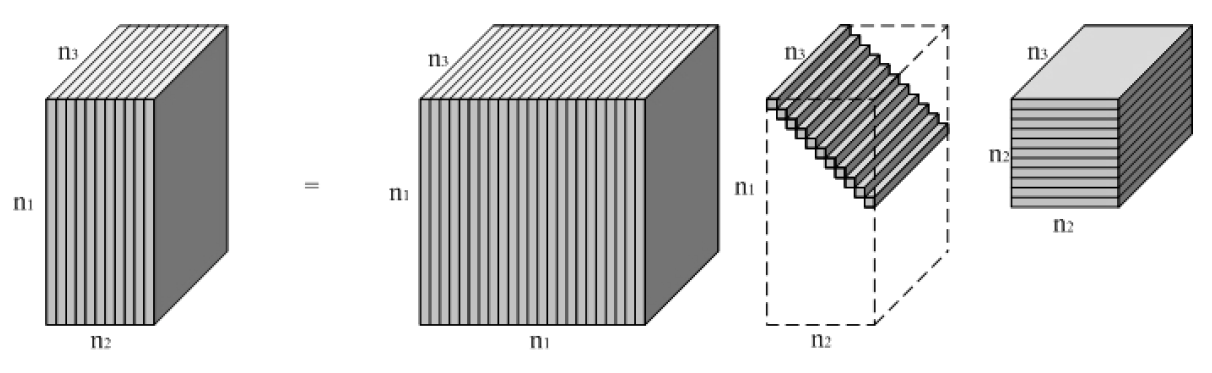
\includegraphics[width=0.8\textwidth]{figs/tsvd.png}
\vskip -2ex
\caption{The t-SVD of an $n_1 \times n_2 \times n_3$ tensor.}
\label{fig1}
\end{figure}
\end{frame}

%------------------------------------------------

\begin{frame}{t-SVD}
\begin{algorithm}[H] 
\caption{t-SVD} 
\label{alg1} 
\begin{algorithmic}[1] 
\Require 
Tensor $\mathcal{A} \in \mathbb{R}^{n_1 \times n_2 \times n_3}$; 
\Ensure 
$\mathcal{U} \in \mathbb{R}^{n_1 \times n_1 \times n_3}$, $\mathcal{S} \in \mathbb{R}^{n_1 \times n_2 \times n_3}$ and $\mathcal{V} \in \mathbb{R}^{n_2 \times n_2 \times n_3}$;

\State $\hat{\mathcal{A}} := \texttt{fft}(\mathcal{A},[],3)$;
\For{$i=1$ to $n_3$}
\State $[U,S,V]=\texttt{SVD}(\hat{\mathcal{A}}(:,:,i))$; 
\State $\hat{\mathcal{U}}(:,:,i):=U$;
\State $\hat{\mathcal{S}}(:,:,i):=S$;
\State $\hat{\mathcal{V}}(:,:,i):=V$;
\EndFor
\State $\mathcal{U}:=\texttt{ifft}(\hat{\mathcal{U}},[],3)$;
\State $\mathcal{S}:=\texttt{ifft}(\hat{\mathcal{S}},[],3)$;
\State $\mathcal{V}:=\texttt{ifft}(\hat{\mathcal{V}},[],3)$;
\end{algorithmic} 
\end{algorithm}

\end{frame}

%------------------------------------------------
\begin{frame}{t-SVD}
\textbf{Example 2}. Take the tensor $\mathcal{A} \in \mathbb{R}^{3\times 2 \times 2}$ same in Example 1. We have the Fourier transformation of $\mathcal{A}$
$$
\hat{\mathcal{A}} = 
\texttt{fold}\left(
\left[\begin{array}{cc}
-1 & 1\\
-2 & 9\\
-1 & 2\\
\hline
3 & -1\\
2 & -5\\
-1 & 4
\end{array}\right]\right).
$$
Now compute the $i=1$-th frontal face's SVD using $[U,S,V]=\texttt{SVD}(\hat{\mathcal{A}}(:,:,1))$.
$$
\hat{\mathcal{U}}(:,:,1):=U=\left[\begin{array}{ccc}
   -0.1268  &  0.8066 & -0.5774\\
   -0.9653  & -0.2343  & -0.1155\\
   -0.2284  &  0.5427  &  0.8083
\end{array}\right],
$$
\end{frame}

\begin{frame}{t-SVD}
$$
\hat{\mathcal{S}}(:,:,1):=S=\left[\begin{array}{cc}
    9.5487  &       0\\
         0  &  0.9070\\
         0  &       0
\end{array}\right],
$$
$$
\hat{\mathcal{V}}(:,:,1):=V=\left[\begin{array}{cc}
    0.2394  & -0.9709\\
   -0.9709  & -0.2394
\end{array}\right].
$$
Next, we can use the same method to get $\hat{\mathcal{U}}(:,:,2)$, $\hat{\mathcal{S}}(:,:,2)$ and $\hat{\mathcal{V}}(:,:,2)$. Last, compute the inverse Fourier transformation of $\hat{\mathcal{U}}$, $\hat{\mathcal{S}}$ and $\hat{\mathcal{V}}$, obtaining $\mathcal{U}$, $\mathcal{S}$ and $\mathcal{V}$.
\end{frame}

%------------------------------------------------
\begin{frame}{t-SVD}
$$
\begin{aligned}
\mathcal{U}&=\texttt{ifft}(\hat{\mathcal{U}},[],3)\\
&=\texttt{ifft}(\texttt{fold}\left(
\left[\begin{array}{ccc}
   -0.1268  &  0.8066 & -0.5774\\
   -0.9653  & -0.2343  & -0.1155\\
   -0.2284  &  0.5427  &  0.8083\\
\hline
   -0.3089  &  0.9351  & -0.1735\\
   -0.7600  & -0.1330  &  0.6361\\
    0.5718  &  0.3284  &  0.7518
\end{array}\right]\right),[],3)\\
&=\texttt{fold}\left(
\left[\begin{array}{ccc}
   -0.2178  &  0.8709 &  -0.3754\\
   -0.8626  & -0.1837  &  0.2603\\
    0.1717  &  0.4355  &  0.7800\\
\hline
    0.0911  & -0.0643  & -0.2019\\
   -0.1026  & -0.0507  & -0.3758\\
   -0.4001  &  0.1072  &  0.0282
\end{array}\right]\right).
\end{aligned}
$$

\end{frame}

%------------------------------------------------
\begin{frame}{t-SVD}
$$
\begin{aligned}
\mathcal{S}&=\texttt{ifft}(\hat{\mathcal{S}},[],3)\\
&=\texttt{ifft}(\texttt{fold}\left(
\left[\begin{array}{cc}
    9.5487  &       0\\
         0  &  0.9070\\
         0  &       0\\
\hline
    7.0727  &       0\\
         0  &  2.4448\\
         0  &       0
\end{array}\right]\right),[],3)\\
&=\texttt{fold}\left(
\left[\begin{array}{cc}
    8.3107  &       0\\
         0  &  1.6759\\
         0  &       0\\
\hline
    1.2380  &       0\\
         0  & -0.7689\\
         0  &       0
\end{array}\right]\right).
\end{aligned}
$$

\end{frame}

%------------------------------------------------
\begin{frame}{t-SVD}
$$
\begin{aligned}
\mathcal{V}&=\texttt{ifft}(\hat{\mathcal{V}},[],3)\\
&=\texttt{ifft}(\texttt{fold}\left(
\left[\begin{array}{cc}
    0.2394  & -0.9709\\
   -0.9709  & -0.2394\\
\hline
   -0.4268  &  0.9044\\
    0.9044  &  0.4268
\end{array}\right]\right),[],3)\\
&=\texttt{fold}\left(
\left[\begin{array}{cc}
   -0.0937  & -0.0333\\
   -0.0333  &  0.0937\\
\hline
    0.3331  & -0.9376\\
   -0.9376  & -0.3331
\end{array}\right]\right).
\end{aligned}
$$

\end{frame}

%------------------------------------------------
\section{Tensor Composition}
%------------------------------------------------

\begin{frame}{Tensor Composition}
\begin{algorithm}[H] 
\caption{Tensor Composition} 
\label{alg2} 
\begin{algorithmic}[1] 
\Require 
$\mathcal{U} \in \mathbb{R}^{n_1 \times n_1 \times n_3}$, $\mathcal{S} \in \mathbb{R}^{n_1 \times n_2 \times n_3}$ and $\mathcal{V} \in \mathbb{R}^{n_2 \times n_2 \times n_3}$;
\Ensure 
$\mathcal{A} \in \mathbb{R}^{n_1 \times n_2 \times n_3}$; 
\State $\hat{\mathcal{U}}:=\texttt{fft}(\mathcal{U},[],3)$;
\State $\hat{\mathcal{S}}:=\texttt{fft}(\mathcal{S},[],3)$;
\State $\hat{\mathcal{V}}:=\texttt{fft}(\mathcal{V},[],3)$;
\For{$i=1$ to $n_3$}
\State $U:=\hat{\mathcal{U}}(:,:,i)$;
\State $S:=\hat{\mathcal{S}}(:,:,i)$;
\State $V:=\hat{\mathcal{V}}(:,:,i)$;
\State $\hat{\mathcal{A}}(:,:,i)=USV^T$; 
\EndFor
\State $\mathcal{A} := \texttt{ifft}(\hat{\mathcal{A}},[],3)$;
\end{algorithmic} 
\end{algorithm}
\end{frame}

%------------------------------------------------

\begin{frame}
\Huge{\centerline{The End}}
\end{frame}

%----------------------------------------------------------------------------------------

\end{document}